% Provenance (never printed): old seconde/premiere S material on the
% atmosphere (water vapour, saturation, cloud formation, the vertical motion
% of air) and enseignement scientifique premiere (water cycle); see
% sources/book2/PROVENANCE.md. Every saturation value, lapse rate,
% condensation level and the lee-wind example are computed in
% figdata/grade-10/clouds.py from the IAPWS saturation curves; the soundings
% are invented examples, said so in the text.
\chapter{为什么会形成云}\label{ch:g10:why-clouds-form}

夏日的露台上，桌上放着一杯冰水。不到一分钟，
杯子外壁就布满了细小的水珠，杯底还淌出一圈水迹。
这些水并非从玻璃中渗出，而是从空气中析出的：
空气接触到冰冷的杯壁后被冷却，水汽便凝结成了水滴。几个小时之后，
在平原上空数千米处，同样的过程以更大的规模出现：
暖空气泡上升、降温，到达某一高度时，它所携带的水汽
便凝结成扁平底部的白色云团，即积云。本章将解释
空气能容纳多少水汽、上升的空气为何会降温、
云在多高处形成、为何有些日子云层低平、
另一些日子云团却直冲云霄形成雷暴，以及微小的云滴如何变成雨
和雪。

\begin{omfigure}

\includegraphics[width=0.5\linewidth]{images/book2/ai/g10-cold-glass.jpg}

{\small 夏日露台上的一杯冰水：杯子外壁形成水珠，
这是因为接触杯壁的空气被冷却。}
\end{omfigure}

\begin{recall}
云由微小的水滴或冰晶组成；按形状和高度可将云分为若干类，
云会带来雨、雪和冰雹，可用雨量计测量（第 1 册，四年级）。
在大气最低层中，气温随高度增加而降低，
平均每千米约降低 \qty{6.5}{\degreeCelsius}，
这就是环境递减率；锋将不同温度的气团分隔开来（第 1 册，八年级）。
气压随高度降低（见物理分册）。
水会蒸发和凝结，
蒸发吸收\omterm{def:g10:earth-energy-budget:latent-heat}{潜热}，凝结时又将\omterm{def:g10:earth-energy-budget:latent-heat}{潜热}释放出来，
见物理分册及
\cref{ch:g10:earth-energy-budget}）。
\end{recall}
% ledger: nasa:grc-atmosphere

\section{水汽与饱和}

空气中总含有一些水汽，它是一种看不见的气体。空气所能容纳的
水汽多少，首先取决于其温度。

\begin{definition}[饱和；相对湿度]\label{def:g10:why-clouds-form:humidity}
当空气所含水汽的质量达到其在该温度下所能容纳的最大值时，
空气称为\emph{饱和}\index{饱和}的，此时的水汽质量称为\emph{饱和含水量}；
多余的水汽会凝结成液滴。空气的\emph{相对湿度}\index{相对湿度}是指，
在相同温度和压强下，空气的水汽含量
与其饱和含水量之比，
并以百分数表示。
\end{definition}

这里以每千克干空气所含水汽的克数（\unit{g/kg}）来表示空气的含水量：
一团上升或下降而既不获得也不失去水分的空气，
其含水量保持不变，即使它膨胀了。

\begin{omfigure}
\begin{tikzpicture}
\begin{axis}[omrecord, width=0.88\linewidth, height=6.2cm, xmin=-10, xmax=40,
  ymin=0, ymax=50, xlabel={温度（\unit{\degreeCelsius}）},
  ylabel={饱和含水量（\unit{g/kg}）}, xtick={-10,0,...,40},
  tick label style={font=\small}, label style={font=\small}]
\addplot[omDef!85!black, thick] table[x=T_C, y=ws_gkg] {figdata/out/grade-10-clouds-sat.dat};
\addplot[only marks, mark=*, mark size=1.8pt, omThm!85!black] coordinates {(28,11.37)};
\addplot[only marks, mark=o, mark size=1.8pt, omThm!85!black] coordinates {(16,11.37)};
\draw[->, omThm!85!black, thick] (axis cs:27.2,11.37) -- (axis cs:16.9,11.37);
\node[anchor=north, font=\footnotesize, omThm!85!black] at (axis cs:28,10.6) {\qty{28}{\degreeCelsius}时的空气};
\node[anchor=south east, font=\footnotesize, omThm!85!black] at (axis cs:15.5,12.2) {露点};
\node[anchor=south east, font=\footnotesize, omDef!85!black, align=right] at (axis cs:31,34) {曲线上方：\\水汽凝结};
\node[anchor=south west, font=\footnotesize, omDef!85!black] at (axis cs:31,2.5) {未饱和};
\node[anchor=north west, font=\footnotesize, omDef!85!black] at (axis cs:34,31.5) {饱和};
\end{axis}
\end{tikzpicture}

{\small 在海平面气压下，每千克空气所能容纳的最大水汽质量
随温度的变化曲线（针对液态水，依据国际标准水性质计算得出）。
\qty{28}{\degreeCelsius}时的空气含有 \qty{11.4}{g/kg} 水汽（实心点），
远未达到\omterm{def:g10:why-clouds-form:humidity}{饱和}；若在不损失水分的情况下将其冷却，
则在 \qty{16}{\degreeCelsius}时达到\omterm{def:g10:why-clouds-form:humidity}{饱和}（空心圆）。}
\end{omfigure}
% ledger: iapws:vapour-pressure, ciaaw:abridged-2024, earth:Mmol, const:R (computed in figdata/grade-10/clouds.py)

该曲线陡然上升：\qty{0}{\degreeCelsius}时为 \qty{3.8}{g/kg}，
\qty{20}{\degreeCelsius}时为 \qty{14.7}{g/kg}，\qty{30}{\degreeCelsius}时为 \qty{27.2}{g/kg}。
气温每升高 \qty{10}{\degreeCelsius}，空气所能容纳的水分几乎翻一番。
这就是热带空气能带来倾盆大雨的原因，
而极地冬季的空气即使\omterm{def:g10:why-clouds-form:humidity}{饱和}，
所含水分也几乎为零。

\begin{definition}[露点]\label{def:g10:why-clouds-form:dew-point}
空气的\emph{露点}\index{露点}是指，
在保持其含水量和压强不变的条件下，
将空气冷却至其达到\omterm{def:g10:why-clouds-form:humidity}{饱和}时的温度。
\end{definition}

\begin{method}[由表格求相对湿度与露点]\label{met:g10:why-clouds-form:table}
\begin{enumerate}
  \item 从表中查出空气温度下的\omterm{def:g10:why-clouds-form:humidity}{饱和}含水量。
  \item \omterm{def:g10:why-clouds-form:humidity}{相对湿度}：用空气的含水量除以该\omterm{def:g10:why-clouds-form:humidity}{饱和}含水量。
  \item \omterm{def:g10:why-clouds-form:dew-point}{露点}：在表中查找
        \omterm{def:g10:why-clouds-form:humidity}{饱和}含水量等于空气含水量的温度。
\end{enumerate}
\end{method}

\begin{example}[夏日清晨]\label{ex:g10:why-clouds-form:morning}
% ledger: iapws:vapour-pressure (values computed in figdata/grade-10/clouds.py)
在 \qty{20}{\degreeCelsius}时，空气含有 \qty{11.4}{g/kg} 水汽。
\qty{20}{\degreeCelsius}时的\omterm{def:g10:why-clouds-form:humidity}{饱和}含水量为 \qty{14.7}{g/kg}，因此\omterm{def:g10:why-clouds-form:humidity}{相对湿度}为
$11.4/14.7 \approx \qty{78}{\percent}$。在 \qty{16}{\degreeCelsius}时，
\omterm{def:g10:why-clouds-form:humidity}{饱和}含水量恰为 \qty{11.4}{g/kg}，这就是\omterm{def:g10:why-clouds-form:dew-point}{露点}。
午后，同样的空气升温至 \qty{28}{\degreeCelsius}
（\omterm{def:g10:why-clouds-form:humidity}{饱和}含水量为 \qty{24.1}{g/kg}），其\omterm{def:g10:why-clouds-form:humidity}{相对湿度}仅为 \qty{47}{\percent}——
而空气中的水分并无任何增减。
\end{example}

窗口的玻璃比周围空气的\omterm{def:g10:why-clouds-form:dew-point}{露点}还冷：
与玻璃接触的空气被冷却到\omterm{def:g10:why-clouds-form:dew-point}{露点}以下，于是在玻璃上析出水分。
晴朗的夜晚，草地和汽车车顶通过向天空辐射
红外线而失热，温度比空气更低：其上凝结成露，若低于 \qty{0}{\degreeCelsius} 则结成霜。
当贴近地面的整层空气冷却到\omterm{def:g10:why-clouds-form:dew-point}{露点}时，
空气中直接形成液滴：雾。

\begin{omfigure}
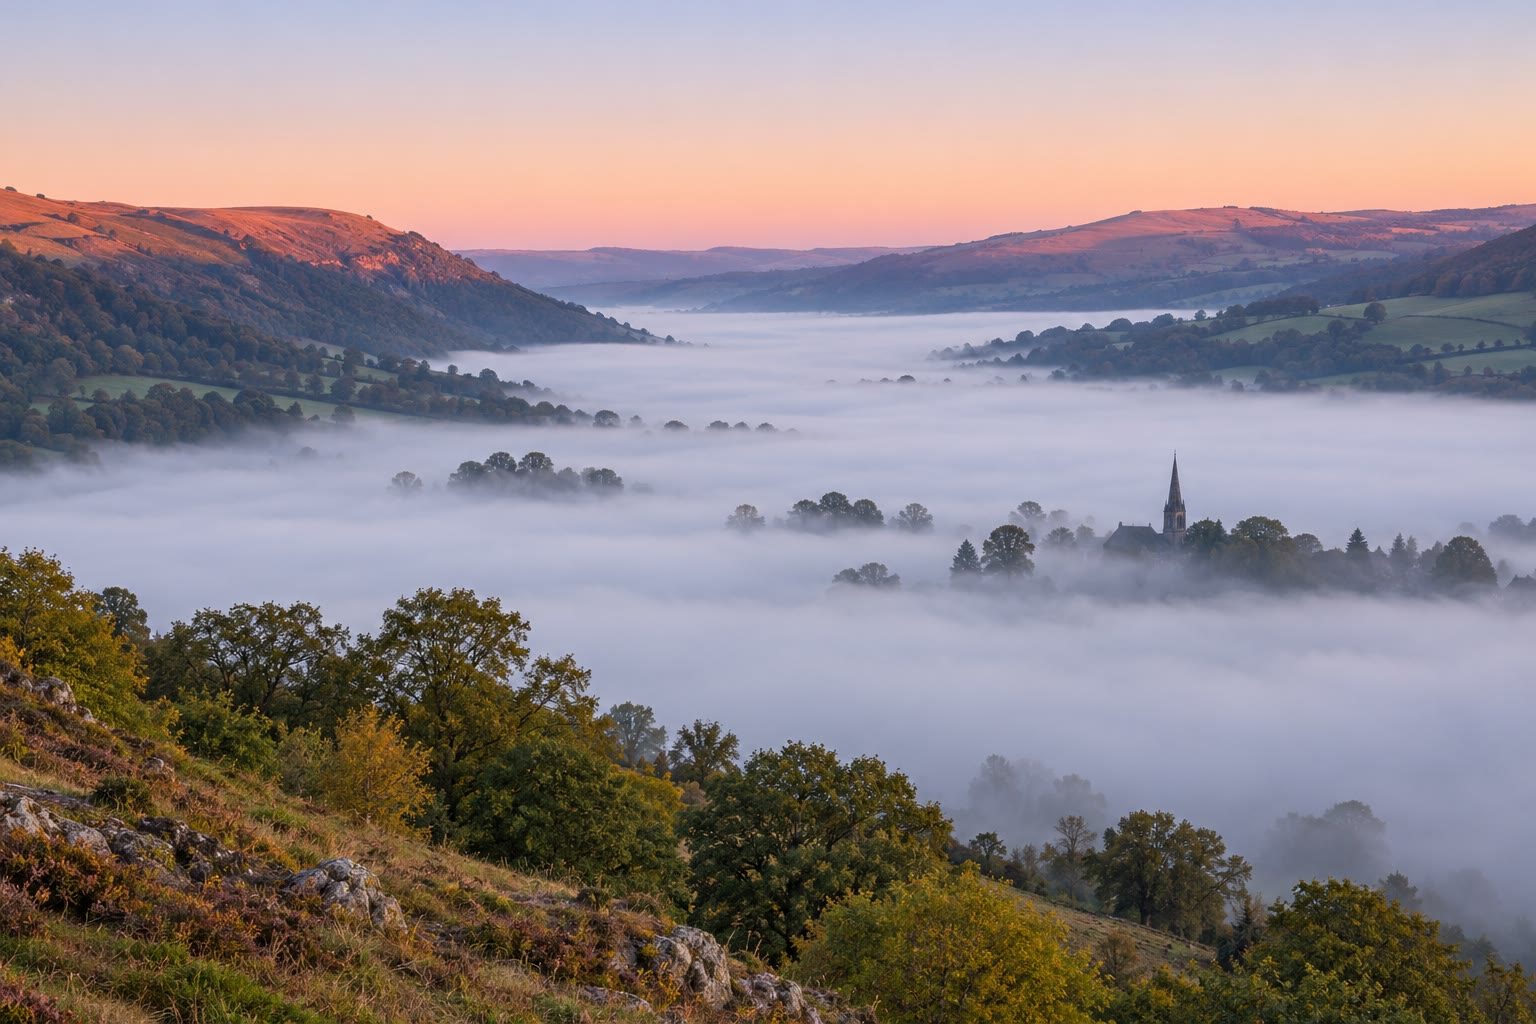
\includegraphics[width=0.75\linewidth]{images/book2/ai/g10-valley-fog.jpg}

{\small 黎明时雾气充满山谷。晴朗的夜间，地面降温，
冷空气沿坡流入谷底，并在那里冷却到
\omterm{def:g10:why-clouds-form:dew-point}{露点}以下。}
\end{omfigure}

\section{上升的空气变冷}

大多数云并非因为空气接触了冷的物体而形成，
而是因为空气上升。气压随高度降低；上升的气块
膨胀，推开周围的空气，做功所需的能量
取自气块自身。

\begin{definition}[绝热冷却；干绝热递减率]\label{def:g10:why-clouds-form:adiabatic}
\emph{绝热冷却}\index{绝热冷却}是指
与外界不交换热量而膨胀的气块所经历的降温。
以这种方式冷却的未\omterm{def:g10:why-clouds-form:humidity}{饱和}上升空气，其降温速率称为
\emph{干绝热递减率}\index{干绝热递减率}，约为每上升一千米
降温 \qty{9.8}{\degreeCelsius}；下沉的空气以相同速率
升温。
\end{definition}

\begin{proposition}[干绝热递减率]\label{prop:g10:why-clouds-form:dry-rate}
\omterm{def:g10:why-clouds-form:adiabatic}{干绝热递减率}为 $g/c_p$，其中 $g = \qty{9.81}{m/s^2}$，$c_p
\approx \qty{1005}{J.kg^{-1}.K^{-1}}$ 为在定压下使一千克
空气升高一度所需的能量：$9.81/1005 \approx
\qty{0.0098}{\degreeCelsius/m}$，即 \qty{9.8}{\degreeCelsius/km}。
（在本阶段不加证明地承认，证明属于物理教材。）
\end{proposition}
% ledger: const:gn, const:R, earth:Mmol (c_p of dry air computed as (7/2)R/M in figdata/grade-10/clouds.py)

气块的\omterm{def:g10:why-clouds-form:dew-point}{露点}随之上升也会降低，但降低得较慢：其含水量保持不变，
而气压下降使水汽稍易达到\omterm{def:g10:why-clouds-form:humidity}{饱和}。对近地面空气的计算表明，
\omterm{def:g10:why-clouds-form:dew-point}{露点}约以每千米 \qty{1.8}{\degreeCelsius} 的速率降低。因此，气块温度
与\omterm{def:g10:why-clouds-form:dew-point}{露点}之间的差距
约以 $9.8 - 1.8 = \qty{8}{\degreeCelsius}$ 的速率缩小，
即每上升一千米缩小上述数值。
% ledger: iapws:vapour-pressure (dew-point rate computed in figdata/grade-10/clouds.py)

\begin{definition}[凝结高度]\label{def:g10:why-clouds-form:condensation-level}
气块的\emph{凝结高度}\index{凝结高度}是指
气块上升时达到\omterm{def:g10:why-clouds-form:humidity}{饱和}的高度。水汽在其上方凝结，
因此凝结高度就是上升空气所形成的云的平坦底部，
即云底。
\end{definition}

\begin{proposition}[凝结高度的确定]\label{prop:g10:why-clouds-form:lcl}
从地面上升、温度为 $T$、\omterm{def:g10:why-clouds-form:dew-point}{露点}为 $T_d$ 的空气
（单位为 \unit{\degreeCelsius}）达到\omterm{def:g10:why-clouds-form:humidity}{饱和}的高度约为
\[
  z = \frac{T - T_d}{8}\ \text{千米} = \qty{125}{m} \times (T - T_d).
\]
\end{proposition}

\begin{proof}
在高度 $z$（以千米计）处，气块温度为 $T - 9.8\,z$，
\omterm{def:g10:why-clouds-form:dew-point}{露点}为 $T_d - 1.8\,z$。二者相等时达到\omterm{def:g10:why-clouds-form:humidity}{饱和}：
$T - 9.8\,z = T_d - 1.8\,z$，于是 $8\,z = T - T_d$，$z = (T - T_d)/8$ 千米。
八分之一千米等于 \qty{125}{m}。
\end{proof}

\begin{example}[一个午后的积云]\label{ex:g10:why-clouds-form:base}
% ledger: iapws:vapour-pressure (exact ascent computed in figdata/grade-10/clouds.py: 1.51 km)
在\cref{ex:g10:why-clouds-form:morning}所描述的午后，地面空气温度为
\qty{28}{\degreeCelsius}，\omterm{def:g10:why-clouds-form:dew-point}{露点}为 \qty{16}{\degreeCelsius}。上升的气泡
在 $125 \times 12 = \qty{1500}{m}$ 处达到\omterm{def:g10:why-clouds-form:humidity}{饱和}，积云的平底
约位于 \qty{1.5}{km} 高处。早晨，温度为 \qty{20}{\degreeCelsius} 时，
同样的空气只会在 $125 \times 4 = \qty{500}{m}$ 处凝结，
因此随着地面升温，
云底在一天之中不断抬升。
\end{example}

\section{稳定空气与不稳定空气}

上升的气块能否继续上升，取决于周围的空气。温度高于周围空气的气块
比它所排开的空气轻，因而像热气球一样上升；温度低于周围空气的气块
则下沉回落。

\begin{definition}[稳定空气；不稳定空气]\label{def:g10:why-clouds-form:stability}
当向上推动的气块变得比周围空气更冷，从而下沉回原处时，
这种空气称为\emph{稳定空气}\index{稳定空气}。
当气块变得比周围空气更暖，并能自行继续上升时，
这种空气称为\emph{不稳定空气}\index{不稳定空气}。
\end{definition}

只要气块未\omterm{def:g10:why-clouds-form:humidity}{饱和}，上升的气块便以\omterm{def:g10:why-clouds-form:adiabatic}{干绝热递减率}降温，即每千米
\qty{9.8}{\degreeCelsius}。一旦\omterm{def:g10:why-clouds-form:humidity}{饱和}，降温便减慢：凝结向气块
释放\omterm{def:g10:earth-energy-budget:latent-heat}{潜热}。计算表明，近地面温暖空气中的降温率约为每千米
\qty{4.7}{\degreeCelsius}，在 \qty{0}{\degreeCelsius} 时约为 \num{5.8}，
而在较高处的寒冷空气中更大，那里可凝结的水汽已所剩无几；
这一数值称为\omterm{def:g10:why-clouds-form:humidity}{饱和}递减率。
（其公式在大学教材中推导。）
% ledger: nist:water-latent, iapws:vapour-pressure (saturated rates computed in figdata/grade-10/clouds.py)

\begin{method}[这种空气是否稳定？]\label{met:g10:why-clouds-form:stable}
\begin{enumerate}
  \item 求出周围空气温度随高度下降的快慢
        （即环境递减率，由探空气球测得）。
  \item 将其与气块的降温速率相比较：\omterm{def:g10:why-clouds-form:condensation-level}{凝结高度}以下为\omterm{def:g10:why-clouds-form:adiabatic}{干绝热递减率}，
        约 \qty{9.8}{\degreeCelsius/km}；\omterm{def:g10:why-clouds-form:condensation-level}{凝结高度}以上为\omterm{def:g10:why-clouds-form:humidity}{饱和}递减率，
        约 \qty{5}{\degreeCelsius/km}。
  \item 若周围空气降温比气块慢，则气块最终变得更冷：稳定；
        若周围空气降温更快，则气块最终变得更暖：不稳定。
        温度随高度\emph{升高}的一层空气非常稳定，
        它像盖子一样阻止空气上升。
\end{enumerate}
\end{method}

当平均递减率约为 \qty{6.5}{\degreeCelsius/km} 时，空气
只要未\omterm{def:g10:why-clouds-form:humidity}{饱和}就稳定（气块降温更快），一旦\omterm{def:g10:why-clouds-form:humidity}{饱和}便不稳定（气块降温较慢）。
这种空气被称为
条件不稳定：除非某种力量将其抬升至
\omterm{def:g10:why-clouds-form:condensation-level}{凝结高度}，否则保持稳定；一旦抬升到\omterm{def:g10:why-clouds-form:condensation-level}{凝结高度}，云便会自行发展。

\begin{omfigure}
\begin{tikzpicture}
\begin{axis}[omrecord, width=0.9\linewidth, height=7.6cm, xmin=-30, xmax=36,
  ymin=0, ymax=6, xlabel={温度 (\unit{\degreeCelsius})}, ylabel={高度 (km)},
  xtick={-30,-20,...,30}, ytick={0,1,...,6},
  legend style={at={(0.02,0.98)}, anchor=north west, font=\footnotesize, draw=black!30, fill=white},
  tick label style={font=\small}, label style={font=\small}]
\fill[omDef!10] (axis cs:-30,1.51) rectangle (axis cs:36,3.96);
\addplot[black!60, thick] table[x=T_C, y=z_km] {figdata/out/grade-10-clouds-envA.dat};
\addlegendentry{探空 A}
\addplot[omProp!90!black, thick, densely dotted] table[x=T_C, y=z_km] {figdata/out/grade-10-clouds-envB.dat};
\addlegendentry{探空 B}
\addplot[omThm!85!black, very thick] table[x=T_C, y=z_km] {figdata/out/grade-10-clouds-parcel.dat};
\addlegendentry{上升气块}
\addplot[omMeth!85!black, thick, dashed] table[x=Td_C, y=z_km] {figdata/out/grade-10-clouds-dew.dat};
\addlegendentry{气块露点}
\draw[black!50, dashed] (axis cs:-30,1.51) -- (axis cs:36,1.51);
\node[anchor=south west, font=\footnotesize] at (axis cs:-29.5,1.53) {凝结高度};
\node[anchor=north east, font=\footnotesize, omDef!80!black] at (axis cs:35.5,3.9) {A 中的云};
\end{axis}
\end{tikzpicture}

{\small 一个自地面上升的气块，初温 \qty{28}{\degreeCelsius}，
\omterm{def:g10:why-clouds-form:dew-point}{露点}为 \qty{16}{\degreeCelsius}（计算值）：它以干绝热速率降温，
直到温度与\omterm{def:g10:why-clouds-form:dew-point}{露点}在 \qty{1.5}{km} 处相等，此后按
较慢的\omterm{def:g10:why-clouds-form:humidity}{饱和}速率降温。图中给出两条虚构的探空曲线：在 A 中，气块
自 \qty{1.5}{km} 向上直至
\qty{4}{km} 附近的暖层都比周围空气暖，两者之间发展出积云（阴影）；在 B 中，
地面以上较暖的空气使气块在各处都比周围空气更冷：
空气稳定，无积云。}
\end{omfigure}
% ledger: iapws:vapour-pressure, nist:water-latent (parcel computed in figdata/grade-10/clouds.py; soundings invented)

空气稳定却仍被抬升——例如越过山脉，或沿锋面——，
形成的云呈扁平的灰色层状铺展，
即层云。空气不稳定时，云向上堆积翻涌，即积云；
不稳定性足够强时，出现雷暴中的积雨云，
其云顶在最低层大气之上的极\omterm{def:g10:why-clouds-form:stability}{稳定空气}中
铺展成铁砧状。

\begin{omfigure}
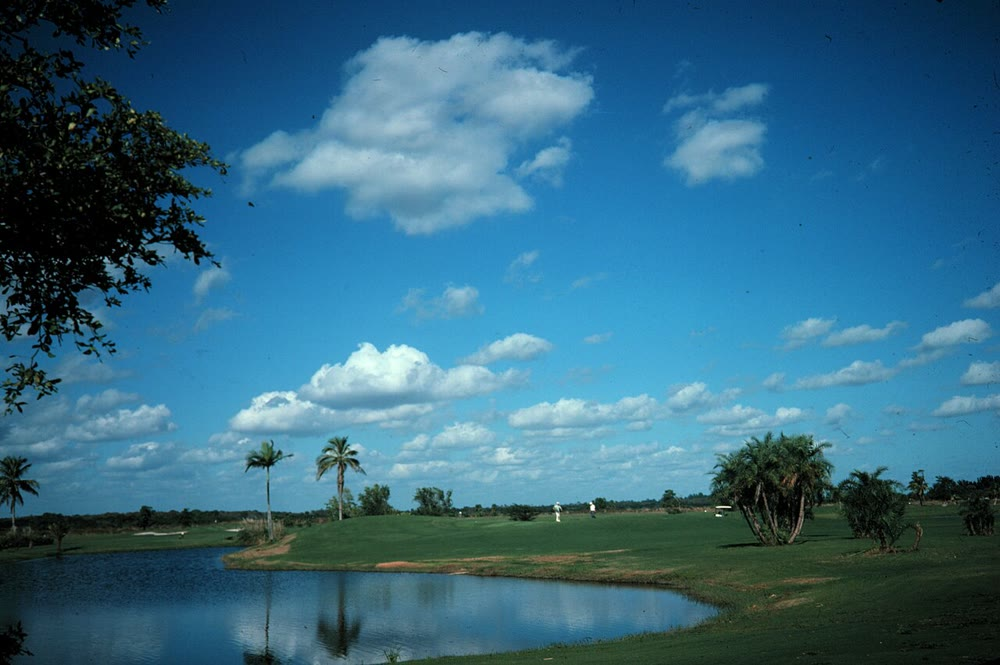
\includegraphics[height=4.5cm]{images/book2/g10-noaa-fair-weather-cumulus.jpg}\hspace{0.6em}%
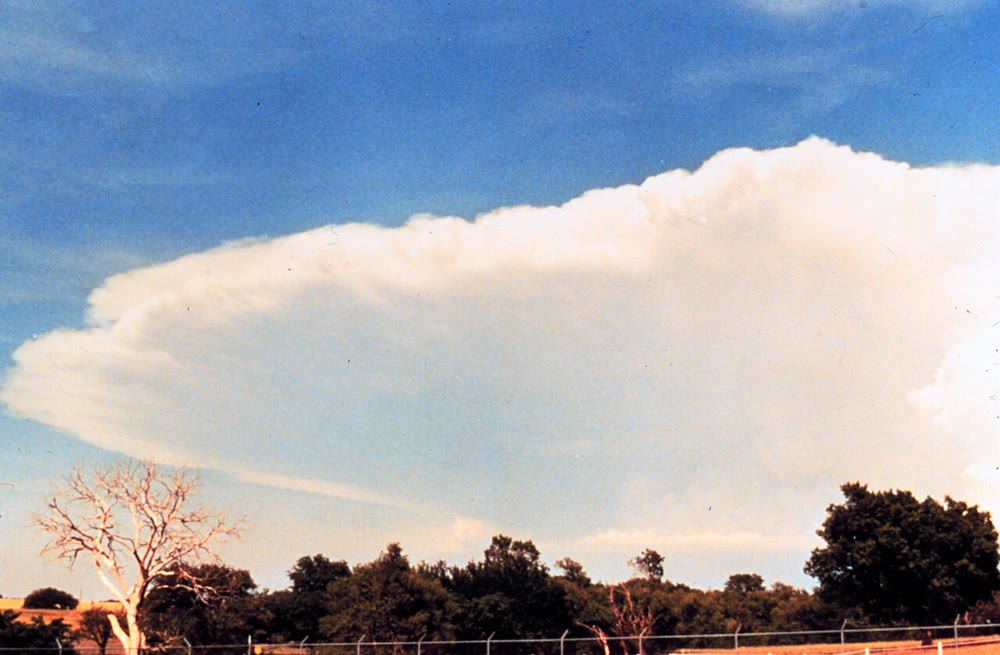
\includegraphics[height=4.5cm]{images/book2/g10-noaa-cumulonimbus-anvil.jpg}

{\small 左：佛罗里达上空的晴天积云，云底平坦，位于
其\omterm{def:g10:why-clouds-form:condensation-level}{凝结高度}。照片：Ralph F. Kresge, NOAA（公有领域）。
右：雷暴早期阶段积雨云的铁砧状云顶。
照片：NOAA National Severe Storms Laboratory（公有领域）。}
\end{omfigure}

\section{抬升空气的四种方式}

空气上升有四种原因。
\begin{itemize}
  \item \textbf{下方加热。} 晴天时，地面加热其上方空气；
        暖空气泡从最热的地块升起，这些
        形成午后的积云。
  \item \textbf{地形抬升。} 迎着山脉吹来的风被迫
        沿山坡向上爬升。
  \item \textbf{锋面抬升。} 暖、冷气团相遇时，较轻的暖
        空气爬升到冷空气之上，或冷空气楔入其下（参见
        第 1 册，八年级）。
  \item \textbf{汇聚抬升。} 近地面的风相互汇聚时，空气
        别无出路，只能上升，例如赤道附近的上升气流带，
        以及低压中心处的上升气流。
\end{itemize}

\begin{method}[跟踪气块越过山脉]\label{met:g10:why-clouds-form:mountain}
\begin{enumerate}
  \item 用 125 米法则求出\omterm{def:g10:why-clouds-form:condensation-level}{凝结高度}；在此之下，
        气块以 \qty{9.8}{\degreeCelsius/km} 降温。
  \item 自\omterm{def:g10:why-clouds-form:condensation-level}{凝结高度}至山脊，气块按\omterm{def:g10:why-clouds-form:humidity}{饱和}速率降温；凝结出的水
        在迎风坡以雨或雪的形式落下。
  \item 越过山脊后，气块下沉且未\omterm{def:g10:why-clouds-form:humidity}{饱和}，
        沿途以 \qty{9.8}{\degreeCelsius/km} 的速率升温。
\end{enumerate}
\end{method}

\begin{example}[背风坡的暖干风]\label{ex:g10:why-clouds-form:lee}
% ledger: iapws:vapour-pressure, nist:water-latent (all values computed in figdata/grade-10/clouds.py)
空气位于海平面，温度为 \qty{20}{\degreeCelsius}，\omterm{def:g10:why-clouds-form:dew-point}{露点}为
\qty{12}{\degreeCelsius}，被吹过一道高 \qty{2500}{m} 的山脊。它
在 $125 \times 8 = \qty{1000}{m}$ 处达到\omterm{def:g10:why-clouds-form:humidity}{饱和}，温度约为
\qty{10}{\degreeCelsius}。自此至山脊，它以\omterm{def:g10:why-clouds-form:humidity}{饱和}速率降温
，降至约 \qty{2}{\degreeCelsius}，并以雨的形式损失约三分之一的
水分（由 \num{8.7} 减至 \qty{6.0}{g/kg}）。翻过山脊后，
它沿 \qty{2.5}{km} 的路程以干绝热速率升温，到达平原时温度约为
\qty{27}{\degreeCelsius}，比出发时高 7 度，\omterm{def:g10:why-clouds-form:humidity}{相对湿度}为
约 \qty{27}{\percent}。这种温暖干燥的风常见于
许多山脉的背风坡上。
\end{example}

\begin{omfigure}
\begin{tikzpicture}[font=\footnotesize, >={Stealth[length=2mm]}]
  \fill[omExo!30] (0,0) -- (3.5,0.3) -- (6,3.0) -- (8.5,0.3) -- (12,0) -- (12,-0.25) -- (0,-0.25) -- cycle;
  \draw[thick, black!70] (0,0) -- (3.5,0.3) -- (6,3.0) -- (8.5,0.3) -- (12,0);
  \draw[black!40, dashed] (0,1.2) -- (4.6,1.2);
  \node[anchor=south west, black!60, align=left] at (0.1,1.22) {凝结高度，\qty{1000}{m}};
  \foreach \x in {3.62,3.86,4.1} \draw[omDef!60] (\x,1.2) -- (\x-0.06,{0.3+(\x-0.06-3.5)*1.08+0.04});
  \pic[scale=1.1, transform shape] at (4.6,1.22) {puffycloud};
  \pic[scale=0.9, transform shape] at (5.0,2.2) {puffycloud};
  \draw[->, thick, omDef!80!black] (0.2,0.25) -- (2.8,0.5) .. controls (3.6,0.75) .. (4.4,1.7) -- (5.4,2.9) .. controls (5.8,3.4) and (6.2,3.4) .. (6.6,2.9) -- (7.6,1.7) .. controls (8.4,0.75) .. (9.2,0.5) -- (11.8,0.25);
  \node[anchor=east, align=right] at (3.4,2.15) {\qty{10}{\degreeCelsius}，饱和};
  \node[anchor=south, align=center] at (6.0,3.45) {山脊 \qty{2500}{m}：\qty{2}{\degreeCelsius}};
  \node[anchor=west, align=left] at (7.75,2.1) {下沉并升温 \\速率 \qty{9.8}{\degreeCelsius/km}};
  \node[anchor=north, align=center] at (1.0,-0.3) {\qty{20}{\degreeCelsius}\\露点 \qty{12}{\degreeCelsius}};
  \node[anchor=north, align=center] at (11.0,-0.3) {\qty{27}{\degreeCelsius}\\露点 \qty{6}{\degreeCelsius}};
  \node[anchor=north, black!60] at (4.0,-0.3) {迎风坡：降雨};
  \node[anchor=north, black!60] at (8.2,-0.3) {背风坡：干燥};
\end{tikzpicture}

{\small 一团空气越过山脊（温度为计算值；
竖直比例夸大）。它以\omterm{def:g10:why-clouds-form:adiabatic}{干绝热递减率}冷却至\omterm{def:g10:why-clouds-form:condensation-level}{凝结高度}，
其上以较慢的\omterm{def:g10:why-clouds-form:humidity}{饱和}递减率冷却，以雨的形式失去水分，并
以\omterm{def:g10:why-clouds-form:adiabatic}{干绝热递减率}沿背风坡一路升温至坡底。}
\end{omfigure}

\section{从云滴到雨和雪}

在十分洁净的空气中，水蒸气不易凝结。云滴
形成于物质微粒之上。

\begin{definition}[凝结核]\label{def:g10:why-clouds-form:nucleus}
称\emph{凝结核}\index{凝结核}为悬浮在空气中的微小颗粒，
——如一粒海盐、尘埃、烟或烟灰——，水汽
在其上凝结成云滴。
\end{definition}

典型\omterm{def:g10:why-clouds-form:nucleus}{凝结核}的直径约为 \qty{0.0002}{mm}，云滴约为
\qty{0.02}{mm}，毛毛雨滴为 \qty{0.5}{mm}，雨滴约为
\qty{2}{mm}。雨滴的直径是云滴的一百倍，因此其
体积为云滴的 $100^3$ 倍：一百万个云滴合成一个雨滴。云滴极小，
即使最弱的上升气流也能使其悬浮于空中；要使雨降落，云滴必须长大百倍。
% ledger: jpl:drop-sizes

\begin{omfigure}
\begin{tikzpicture}
\begin{axis}[width=0.9\linewidth, height=3.4cm, xmode=log, xmin=1e-4, xmax=10,
  ymin=0, ymax=1, axis y line=none, axis x line*=bottom,
  xlabel={直径（mm），对数刻度}, tick label style={font=\small},
  label style={font=\small}, clip=false]
\addplot[only marks, mark=*, omDef!85!black, mark size=2.5pt] coordinates {(0.0002,0.3) (0.02,0.3) (0.5,0.3) (2,0.3)};
\node[anchor=south, font=\footnotesize, align=center] at (axis cs:0.0002,0.42) {凝结核};
\node[anchor=south, font=\footnotesize, align=center] at (axis cs:0.02,0.42) {云滴};
\node[anchor=south, font=\footnotesize, align=center] at (axis cs:0.5,0.42) {毛毛雨};
\node[anchor=south, font=\footnotesize, align=center] at (axis cs:2,0.42) {雨滴};
\end{axis}
\end{tikzpicture}

{\small 典型尺寸，比例尺上每一级为前一级的十倍，
即每个对象的直径约为前一个的一百倍，
毛毛雨除外。数据来源：NASA Jet Propulsion Laboratory。}
\end{omfigure}

有两种过程使它们增长。

\begin{definition}[暖雨过程；冰晶过程]\label{def:g10:why-clouds-form:rain-processes}
在\emph{暖雨过程}\index{暖雨过程}中，云中较大的
云滴下落速度快于小云滴，与之碰撞并
合并，在下落中长大。在\emph{冰晶
过程}\index{冰晶过程}中，云中温度低于
\qty{0}{\degreeCelsius}的部分，冰晶与过冷云滴（
即 \qty{0}{\degreeCelsius} 以下的液态水）共存时，冰晶通过夺取
云滴蒸发出的蒸气而增长；它们以雪花形式下落，若下方空气温暖，便融化成
雨滴。
\end{definition}

\omterm{def:g10:why-clouds-form:rain-processes}{冰晶过程}之所以有效，是因为同温度下冰面上的\omterm{def:g10:why-clouds-form:humidity}{饱和}含水量
低于水面：在
\qty{-10}{\degreeCelsius}时，水面上的\omterm{def:g10:why-clouds-form:humidity}{饱和}蒸气压为 \qty{287}{Pa}，
冰面上为 \qty{260}{Pa}。对于云滴已\omterm{def:g10:why-clouds-form:humidity}{饱和}的空气，
所含蒸气比冰晶所能容纳的多 \qty{10}{\percent}：蒸气在
冰晶上凝结，云滴蒸发以补充这部分蒸气。
% ledger: iapws:vapour-pressure, iapws:melt-subl (computed in figdata/grade-10/clouds.py)

\begin{remark}[潜热助长风暴]\label{rem:g10:why-clouds-form:latent}
云中每凝结一千克水，便向空气释放约
\qty{2.5}{MJ}的热量，即水蒸发时从海洋或地面吸收的\omterm{def:g10:earth-energy-budget:latent-heat}{潜热}
（见\cref{ch:g10:earth-energy-budget}）。这部分热量使\omterm{def:g10:why-clouds-form:humidity}{饱和}
递减率小于\omterm{def:g10:why-clouds-form:adiabatic}{干绝热递减率}，并维持积雨云上升；
\cref{ch:g10:storms-and-cyclones}将讨论其在最强风暴中的作用。
\end{remark}
% ledger: nist:water-latent

\section{练习}

做这些练习时，请使用下表中的\omterm{def:g10:why-clouds-form:humidity}{饱和}含水量（单位为 \unit{g/kg}，
海平面气压下），以及\omterm{def:g10:why-clouds-form:adiabatic}{干绝热递减率}
\qty{9.8}{\degreeCelsius/km}、\omterm{def:g10:why-clouds-form:dew-point}{露点}下降率 \qty{1.8}{\degreeCelsius/km}
及\omterm{def:g10:why-clouds-form:humidity}{饱和}递减率 \qty{5}{\degreeCelsius/km}。
% ledger: iapws:vapour-pressure (table from figdata/out/grade-10-clouds-sat.dat, rounded)

\begin{center}
\small
\begin{tabular}{l*{11}{c}}
\hline
温度（\unit{\degreeCelsius}）& 0 & 4 & 8 & 10 & 12 & 14 & 16 & 20 & 24 & 28 & 30 \\
\omterm{def:g10:why-clouds-form:humidity}{饱和}含水量（\unit{g/kg}）& 3.8 & 5.0 & 6.7 & 7.6 & 8.7 & 10.0 & 11.4 & 14.7 & 18.9 & 24.1 & 27.2 \\
\hline
\end{tabular}
\end{center}

\begin{exercise}[$\star$]\label{exo:g10:why-clouds-form:1}
定义空气的\omterm{def:g10:why-clouds-form:humidity}{相对湿度}和\omterm{def:g10:why-clouds-form:dew-point}{露点}。
\end{exercise}

\begin{exercise}[$\star$]\label{exo:g10:why-clouds-form:2}
根据上表，给出 \num{0}、\num{10}、
\num{20} 和 \qty{30}{\degreeCelsius}时的\omterm{def:g10:why-clouds-form:humidity}{饱和}含水量。每升温
\qty{10}{\degreeCelsius}，\omterm{def:g10:why-clouds-form:humidity}{饱和}含水量大约增至原来的几倍？
\end{exercise}

\begin{exercise}[$\star$]\label{exo:g10:why-clouds-form:3}
温度为 \qty{24}{\degreeCelsius} 的空气含有 \qty{10.0}{g/kg} 的水蒸气。
求其\omterm{def:g10:why-clouds-form:humidity}{相对湿度}和\omterm{def:g10:why-clouds-form:dew-point}{露点}。
\end{exercise}

\begin{exercise}[$\star$]\label{exo:g10:why-clouds-form:4}
解释为什么夏天一杯冰水会“出汗”，而在
冬季室内非常干燥的日子则不会。
\end{exercise}

\begin{exercise}[$\star$]\label{exo:g10:why-clouds-form:5}
说出使空气上升的四种方式，并各举一例。
\end{exercise}

\begin{exercise}[$\star\star$]\label{exo:g10:why-clouds-form:6}
利用\cref{prop:g10:why-clouds-form:lcl}，求
温度为 \qty{30}{\degreeCelsius}、\omterm{def:g10:why-clouds-form:dew-point}{露点}为
\qty{18}{\degreeCelsius} 的空气以及温度为 \qty{22}{\degreeCelsius}、\omterm{def:g10:why-clouds-form:dew-point}{露点}为
\qty{20}{\degreeCelsius} 的空气的云底高度。哪一天可能是阴沉、低云的天气？
\end{exercise}

\begin{exercise}[$\star\star$]\label{exo:g10:why-clouds-form:7}
一团不\omterm{def:g10:why-clouds-form:humidity}{饱和}空气块从地面出发，初温为 \qty{18}{\degreeCelsius}。
若其保持不\omterm{def:g10:why-clouds-form:humidity}{饱和}，则上升 \qty{1}{km} 和 \qty{2}{km}
处的温度各为多少？若其从 \qty{2}{km} 处下沉，
则到达地面时的温度为多少？
\end{exercise}

\begin{exercise}[$\star\star$]\label{exo:g10:why-clouds-form:8}
一次探空气球的观测显示，气温随高度
每千米下降 \qty{4}{\degreeCelsius}。该大气对不\omterm{def:g10:why-clouds-form:humidity}{饱和}气块是否稳定？对\omterm{def:g10:why-clouds-form:humidity}{饱和}气块呢？
在炎热的午后，地面以上的第一千米内
气温下降 \qty{12}{\degreeCelsius}：暖空气泡会发生什么变化？
\end{exercise}

\begin{exercise}[$\star\star$]\label{exo:g10:why-clouds-form:9}
温度为 \qty{20}{\degreeCelsius} 的\omterm{def:g10:why-clouds-form:humidity}{饱和}空气被冷却至
\qty{10}{\degreeCelsius}。每千克空气
中有多少克水凝结？所释放的\omterm{def:g10:earth-energy-budget:latent-heat}{潜热}去向何处？
\end{exercise}

\begin{exercise}[$\star\star$]\label{exo:g10:why-clouds-form:10}
直径为 \qty{0.02}{mm} 的云滴，需要多少个才能组成
一滴直径为 \qty{0.5}{mm} 的毛毛雨？直径为 \qty{2}{mm} 的雨滴又需要多少个？
\end{exercise}

\begin{exercise}[$\star\star$]\label{exo:g10:why-clouds-form:11}
请分步解释，在晴朗、无风的夜晚之后，
黎明时雾为什么形成于山谷而不是山顶。
\end{exercise}

\begin{exercise}[$\star\star\star$]\label{exo:g10:why-clouds-form:12}
\omterm{def:g10:why-clouds-form:adiabatic}{干绝热递减率}为 $a$，\omterm{def:g10:why-clouds-form:dew-point}{露点}下降的速率为 $b$（二者单位均为
\unit{\degreeCelsius/km}）。证明\omterm{def:g10:why-clouds-form:condensation-level}{凝结高度}为
$z = (T - T_d)/(a - b)$。在一座高原上，\omterm{def:g10:why-clouds-form:dew-point}{露点}以
\qty{1.7}{\degreeCelsius/km} 的速率下降时，
“每度 \qty{125}{m}”这一规则会变成什么？
\end{exercise}

\begin{exercise}[$\star\star\star$]\label{exo:g10:why-clouds-form:13}
海平面处温度为 \qty{15}{\degreeCelsius}、\omterm{def:g10:why-clouds-form:dew-point}{露点}为
\qty{11}{\degreeCelsius} 的空气越过一座高 \qty{2000}{m} 的山脊。依据
\cref{met:g10:why-clouds-form:mountain}，求\omterm{def:g10:why-clouds-form:condensation-level}{凝结高度}、该处的温度、
山脊顶的温度，以及
空气到达对面平原时的温度。
\end{exercise}

\begin{exercise}[$\star\star\star$]\label{exo:g10:why-clouds-form:14}
在 \qty{-20}{\degreeCelsius} 时，水面上的\omterm{def:g10:why-clouds-form:humidity}{饱和}水汽压为
\qty{126}{Pa}，冰面上为 \qty{103}{Pa}。以冰面为准，
云滴所在的空气相对于冰面过\omterm{def:g10:why-clouds-form:humidity}{饱和}了百分之多少？与
\qty{-10}{\degreeCelsius} 时相比，并说明\omterm{def:g10:why-clouds-form:rain-processes}{冰晶过程}在云中何处
效果最好。
\end{exercise}

\begin{exercise}[$\star\star\star$]\label{exo:g10:why-clouds-form:15}
周围空气以 \qty{6.5}{\degreeCelsius/km} 的速率降温。一个气块从
与周围空气相同的温度出发，上升 \qty{1}{km}。计算
若气块不\omterm{def:g10:why-clouds-form:humidity}{饱和}，则其温度与周围空气温度之差，
若其\omterm{def:g10:why-clouds-form:humidity}{饱和}，则又为多少。解释“条件
不稳定”一词的含义。
\end{exercise}

\section{问题：平原上的夏日午后}

\begin{problem}[{周末问题——从清晨的湿度到
午后云的云底}]
\label{pb:g10:why-clouds-form:1}
% ledger: iapws:vapour-pressure, nist:water-latent (all results computed in figdata/grade-10/clouds.py or from the rounded data below; the sounding is sounding A, invented)
在一片广阔的平原上，某个夏日，近地面的空气全天
含有 \qty{11.4}{g/kg} 的水汽。早晨温度为 \qty{20}{\degreeCelsius}，
午后为 \qty{28}{\degreeCelsius}。一次探空气球观测
（虚构示例）给出上方空气的温度：

\begin{center}
\small
\begin{tabular}{l*{8}{c}}
\hline
高度（千米） & 0 & 0.5 & 1.0 & 1.5 & 2.5 & 3.5 & 3.6 & 4.0 \\
温度（\unit{\degreeCelsius}） & 28.0 & 23.1 & 18.2 & 13.4 & 6.9 & 0.4 & $-0.3$ & 1.2 \\
\hline
\end{tabular}
\end{center}

\noindent 利用前文的\omterm{def:g10:why-clouds-form:humidity}{饱和}含水量表以及
练习前给出的速率。

\medskip
\noindent\textbf{第一部分——湿度。}
\begin{enumerate}
  \item 给出 \qty{20}{\degreeCelsius} 时的\omterm{def:g10:why-clouds-form:humidity}{饱和}含水量。
  \item 计算早晨的\omterm{def:g10:why-clouds-form:humidity}{相对湿度}。
  \item 求空气的\omterm{def:g10:why-clouds-form:dew-point}{露点}。
  \item 计算午后的\omterm{def:g10:why-clouds-form:humidity}{相对湿度}。
  \item 午后空气是否变得更干燥？说明理由。
\end{enumerate}

\medskip
\noindent\textbf{第二部分——夜间与露水。}
\begin{enumerate}[resume]
  \item 夜间近地面空气降温。露水开始形成时，
        气温为多少？
  \item 若空气降温至 \qty{12}{\degreeCelsius}，每千克空气中
        已有多少克水汽凝结？
  \item 为什么露水先出现在草地和车顶上，
        而不是先在空气中形成？
\end{enumerate}

\medskip
\noindent\textbf{第三部分——探空曲线。}
\begin{enumerate}[resume]
  \item 计算温度在 \num{0} 至 \qty{1.5}{km}
        之间的递减率，并与\omterm{def:g10:why-clouds-form:adiabatic}{干绝热递减率}比较。
  \item 计算温度在 \num{1.5} 至 \qty{3.5}{km} 之间的递减率。
  \item 对未\omterm{def:g10:why-clouds-form:humidity}{饱和}气块而言，\num{1.5} 至 \qty{3.5}{km} 之间的空气是
        否稳定？对\omterm{def:g10:why-clouds-form:humidity}{饱和}气块而言呢？
  \item \num{3.6} 至 \qty{4.0}{km} 之间发生了什么？它对
        上升的云有何影响？
\end{enumerate}

\medskip
\noindent\textbf{第四部分——云底。}
\begin{enumerate}[resume]
  \item 计算午后地面处空气温度与其\omterm{def:g10:why-clouds-form:dew-point}{露点}
        之差。
  \item 计算这团空气中一个气块，
        上升 \qty{1}{km} 后（仍未\omterm{def:g10:why-clouds-form:humidity}{饱和}）的温度和\omterm{def:g10:why-clouds-form:dew-point}{露点}。
  \item 两者之差缩小了多少？其缩小的
        速率是多少？
  \item 证明该速率给出规则“每降一度，云底升高 \qty{125}{m}”。
  \item 上午时云底的高度是多少？
  \item 解释为什么积云云底在白天会升高。
  \item 写出方程，表示气块温度等于
        高度 $z$（单位为 km）处的\omterm{def:g10:why-clouds-form:dew-point}{露点}。
  \item 求解该方程：午后积云的云底位于何高度？
\end{enumerate}
\end{problem}
